\begin{frame}{OMNeT++ und INET}
	\begin{center}
		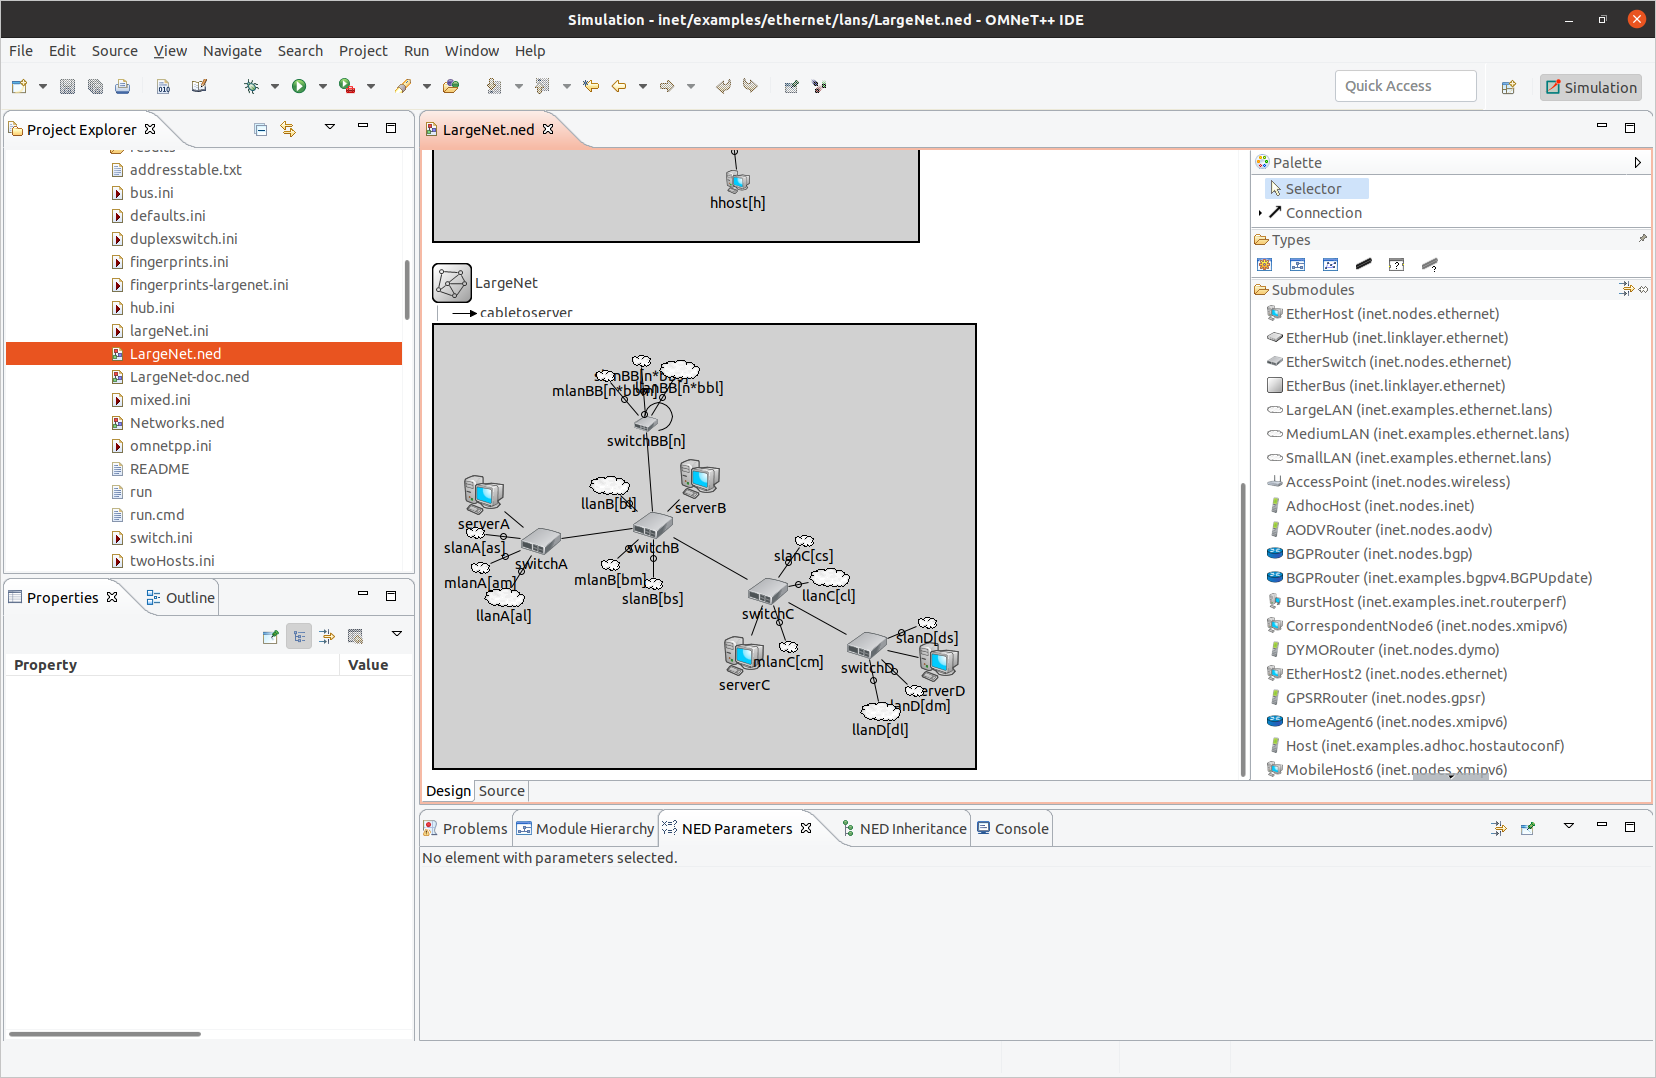
\includegraphics[keepaspectratio,
		width=\paperwidth,
		height=0.8\paperheight]{pic/omnet}
	\end{center}

	\note{
		\begin{itemize}
			\item OMNeT++ besteht aus zwei Teilen
			\begin{itemize}
				\item Simulationskern
				\item IDE
			\end{itemize}
			\item Hier Eclipse IDE
			\item Zu sehen INET
			\item Erweiterung für Netzwerkmodule
			\item OMNeT++ und INET in älterer Version wegen SEA++
			\item SEA++ keine IDE
		\end{itemize}
	}
\end{frame}